% Meridian Multimodal Research Platform -- repository, modalities, and system overview
% Overleaf: New Project > Upload Project > this file (or paste into main.tex).
% Compiler: pdfLaTeX (default). No other files are needed; every figure is drawn with TikZ.
\documentclass[aspectratio=169,11pt]{beamer}

\usepackage[T1]{fontenc}
\usepackage{lmodern}
\usepackage{booktabs}
\usepackage{array}
\usepackage{tabularx}
\usepackage{xcolor}
\usepackage{tikz}
\usetikzlibrary{arrows.meta,positioning,shapes.geometric,fit,calc,backgrounds}

% ---------------------------------------------------------------- theme
\definecolor{ink}{HTML}{1F2A36}
\definecolor{paper}{HTML}{F7F3EC}
\definecolor{sand}{HTML}{E9E1D4}
\definecolor{clay}{HTML}{A8543A}
\definecolor{moss}{HTML}{3D6B45}
\definecolor{slate}{HTML}{5F6B77}
\definecolor{sky}{HTML}{2F5F8A}
\definecolor{plum}{HTML}{76509A}
\definecolor{amber}{HTML}{C08A1E}

\usetheme{default}
\setbeamercolor{background canvas}{bg=paper}
\setbeamercolor{normal text}{fg=ink}
\setbeamercolor{frametitle}{fg=ink}
\setbeamercolor{title}{fg=ink}
\setbeamercolor{subtitle}{fg=clay}
\setbeamercolor{structure}{fg=clay}
\setbeamercolor{alerted text}{fg=clay}
\setbeamercolor{block title}{bg=sand,fg=ink}
\setbeamercolor{block body}{bg=white,fg=ink}
\setbeamerfont{frametitle}{size=\Large,series=\bfseries}
\setbeamerfont{title}{size=\huge,series=\bfseries}
\setbeamerfont{block title}{size=\small,series=\bfseries}
\setbeamertemplate{navigation symbols}{}
\setbeamertemplate{itemize items}{\color{clay}\rule[0.35ex]{0.6ex}{0.6ex}}
\setbeamertemplate{itemize subitem}{\color{slate}--}
\setbeamertemplate{frametitle}{%
  \vspace*{0.5em}\insertframetitle\par
  {\color{clay}\rule{2.2em}{2pt}}%
}
\setbeamertemplate{footline}{%
  \hspace{1em}{\color{slate}\tiny MERIDIAN \quad\textbar\quad \insertsection}\hfill
  {\color{slate}\tiny\insertframenumber\,/\,\inserttotalframenumber}\hspace{1em}\vspace{0.6em}
}
\AtBeginSection[]{%
  \begin{frame}[plain,noframenumbering]
    \vfill
    {\color{clay}\small SECTION \thesection}\par\vspace{0.3em}
    {\color{ink}\Huge\bfseries\insertsection}\par\vspace{0.4em}
    {\color{clay}\rule{3em}{2pt}}
    \vfill
  \end{frame}
}

\newcommand{\code}[1]{{\small\texttt{#1}}}

\tikzset{
  box/.style={draw=ink!70,fill=white,rounded corners=2pt,align=center,font=\small,inner sep=5pt},
  soft/.style={box,fill=sand},
  accent/.style={box,draw=clay,fill=clay!10},
  contact/.style={box,draw=moss,fill=moss!10},
  contactless/.style={box,draw=sky,fill=sky!10},
  context/.style={box,draw=amber,fill=amber!12},
  group/.style={draw=slate!60,dashed,rounded corners=4pt,inner sep=8pt},
  arr/.style={-{Stealth[length=2mm]},ink!80,thick},
  lbl/.style={font=\scriptsize,color=slate,align=center},
}

% Small signal sketch: #1 = y expression in \x (x from 0 to 4.5), #2 = colour, #3 = caption
\newcommand{\sketch}[3]{%
  \begin{tikzpicture}[x=1cm,y=0.9cm]
    \draw[slate!50] (0,0) -- (4.6,0);
    \draw[thick,#2,domain=0:4.5,samples=200] plot (\x,{#1});
    \node[lbl] at (2.3,-0.45) {#3};
  \end{tikzpicture}%
}

% One slide per modality: #1 title, #2 what it measures, #3 hardware and interface, #4 recorded as,
% #5 live checks, #6 derived outputs, #7 figure
\newcommand{\modalityslide}[7]{%
  \begin{frame}{#1}
    \begin{columns}[T]
      \column{0.55\textwidth}
      \small
      \textbf{\color{clay}What it measures and why}\par\vspace{1pt}#2\par\medskip
      \textbf{\color{clay}Hardware and interface}\par\vspace{1pt}#3\par\medskip
      \textbf{\color{clay}Recorded as}\par\vspace{1pt}#4
      \column{0.42\textwidth}
      \footnotesize
      \begin{block}{Live in the instructor console}#5\end{block}
      \begin{block}{Derived in the export}#6\end{block}
      \centering #7
    \end{columns}
  \end{frame}
}

\title{Meridian}
\subtitle{A multimodal data-collection rig for emotion, stress, and contactless physiology}
\author{Your Name}
\institute{IIT Ropar}
\date{\today}

\begin{document}

% ================================================================ title
\begin{frame}[plain]
  \vfill
  {\color{clay}\small MULTIMODAL HUMAN-SUBJECT DATA COLLECTION}\par\vspace{0.6em}
  {\usebeamerfont{title}\usebeamercolor[fg]{title}\inserttitle}\par\vspace{0.3em}
  {\Large\usebeamercolor[fg]{subtitle}\insertsubtitle}\par\vspace{1.2em}
  {\color{clay}\rule{3em}{2pt}}\par\vspace{1em}
  {\normalsize\insertauthor\quad\textbar\quad\insertinstitute\quad\textbar\quad\insertdate}\par
  \vspace{0.4em}{\small\color{slate}Protocol v9 \quad\textbar\quad 12 recorded streams}
  \vfill
\end{frame}

\begin{frame}{Outline}
  \begin{columns}[T]
    \column{0.48\textwidth}
    \begin{enumerate}
      \item What Meridian is
      \item Architecture and repository
      \item The twelve modalities
      \item The study protocol
      \item Subject display
      \item Instructor console
    \end{enumerate}
    \column{0.48\textwidth}
    \begin{enumerate}\setcounter{enumi}{6}
      \item Session engine and storage
      \item Acquisition agent and synchronization
      \item Data output and quality control
      \item Testing and results
    \end{enumerate}
  \end{columns}
\end{frame}

% ================================================================ 1
\section{What Meridian Is}

\begin{frame}{The problem Meridian solves}
  \begin{columns}[T]
    \column{0.55\textwidth}
    \begin{itemize}
      \item A participant watches emotional film clips, rates feelings, answers questionnaires, and performs cognitive tasks and breathing and movement exercises
      \item Contact sensors (ECG, pulse oximeter, EMG, skin conductance, respiration) record reference physiology
      \item Contactless sensors (face video, thermal video, WiFi CSI, audio) record the same moments
      \item Every stimulus, response, and artifact is placed on the \alert{same clock} as every sensor sample
    \end{itemize}
    \column{0.42\textwidth}
    \begin{block}{Research goals}
      \begin{itemize}
        \item Contactless vital signs validated against contact references
        \item Emotion recognition
        \item Stress and cognitive load
        \item A shareable, documented public dataset (30--60 participants)
      \end{itemize}
    \end{block}
  \end{columns}
\end{frame}

\begin{frame}{Three components}
  \centering
  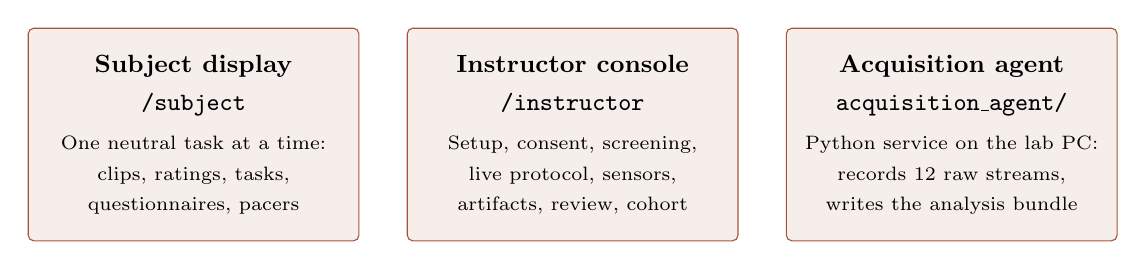
\begin{tikzpicture}[node distance=6mm]
    \node[accent,minimum width=4.2cm,minimum height=2.7cm] (s) {\textbf{Subject display}\\[3pt]\code{/subject}\\[3pt]\scriptsize One neutral task at a time:\\\scriptsize clips, ratings, tasks,\\\scriptsize questionnaires, pacers};
    \node[accent,minimum width=4.2cm,minimum height=2.7cm,right=of s] (i) {\textbf{Instructor console}\\[3pt]\code{/instructor}\\[3pt]\scriptsize Setup, consent, screening,\\\scriptsize live protocol, sensors,\\\scriptsize artifacts, review, cohort};
    \node[accent,minimum width=4.2cm,minimum height=2.7cm,right=of i] (a) {\textbf{Acquisition agent}\\[3pt]\code{acquisition\_agent/}\\[3pt]\scriptsize Python service on the lab PC:\\\scriptsize records 12 raw streams,\\\scriptsize writes the analysis bundle};
  \end{tikzpicture}
  \vspace{0.8em}

  \small The two web portals share one session state on a Cloudflare Worker. The agent talks to the same session over a token-authenticated channel and keeps raw data on the lab computer.
\end{frame}

\begin{frame}{The twelve modalities at a glance}
  \centering
  \resizebox{\textwidth}{!}{%
  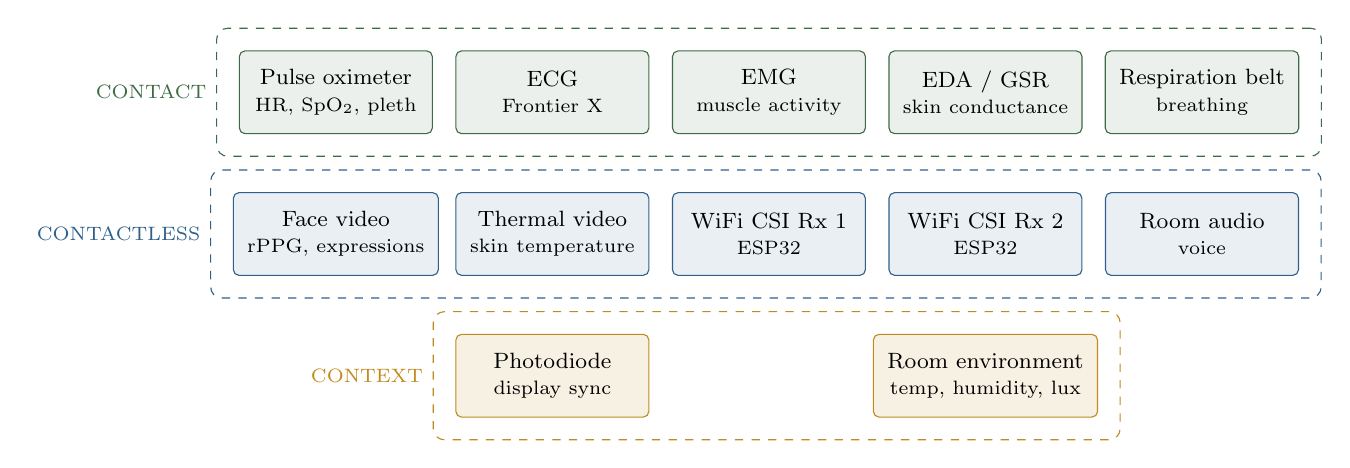
\begin{tikzpicture}[mod/.style={minimum width=2.45cm,minimum height=1.05cm,font=\footnotesize}]
    \node[contact,mod] (oxi) at (0,0) {Pulse oximeter\\\scriptsize HR, SpO$_2$, pleth};
    \node[contact,mod] (ecg) at (2.75,0) {ECG\\\scriptsize Frontier X};
    \node[contact,mod] (emg) at (5.5,0) {EMG\\\scriptsize muscle activity};
    \node[contact,mod] (gsr) at (8.25,0) {EDA / GSR\\\scriptsize skin conductance};
    \node[contact,mod] (resp) at (11,0) {Respiration belt\\\scriptsize breathing};
    \node[contactless,mod] (face) at (0,-1.8) {Face video\\\scriptsize rPPG, expressions};
    \node[contactless,mod] (thermal) at (2.75,-1.8) {Thermal video\\\scriptsize skin temperature};
    \node[contactless,mod] (csi) at (5.5,-1.8) {WiFi CSI Rx 1\\\scriptsize ESP32};
    \node[contactless,mod] (csi2) at (8.25,-1.8) {WiFi CSI Rx 2\\\scriptsize ESP32};
    \node[contactless,mod] (audio) at (11,-1.8) {Room audio\\\scriptsize voice};
    \node[context,mod] (pd) at (2.75,-3.6) {Photodiode\\\scriptsize display sync};
    \node[context,mod] (env) at (8.25,-3.6) {Room environment\\\scriptsize temp, humidity, lux};
    \begin{scope}[on background layer]
      \node[group,draw=moss,fit=(oxi)(resp),label={[lbl,text=moss]left:CONTACT}] {};
      \node[group,draw=sky,fit=(face)(audio),label={[lbl,text=sky]left:CONTACTLESS}] {};
      \node[group,draw=amber,fit=(pd)(env),label={[lbl,text=amber]left:CONTEXT}] {};
    \end{scope}
  \end{tikzpicture}%
  }
  \vspace{0.4em}

  \small Contact streams are the references; contactless streams are what the dataset validates; context streams make timing and conditions reproducible.
\end{frame}

% ================================================================ 2
\section{Architecture and Repository}

\begin{frame}{Architecture}
  \centering
  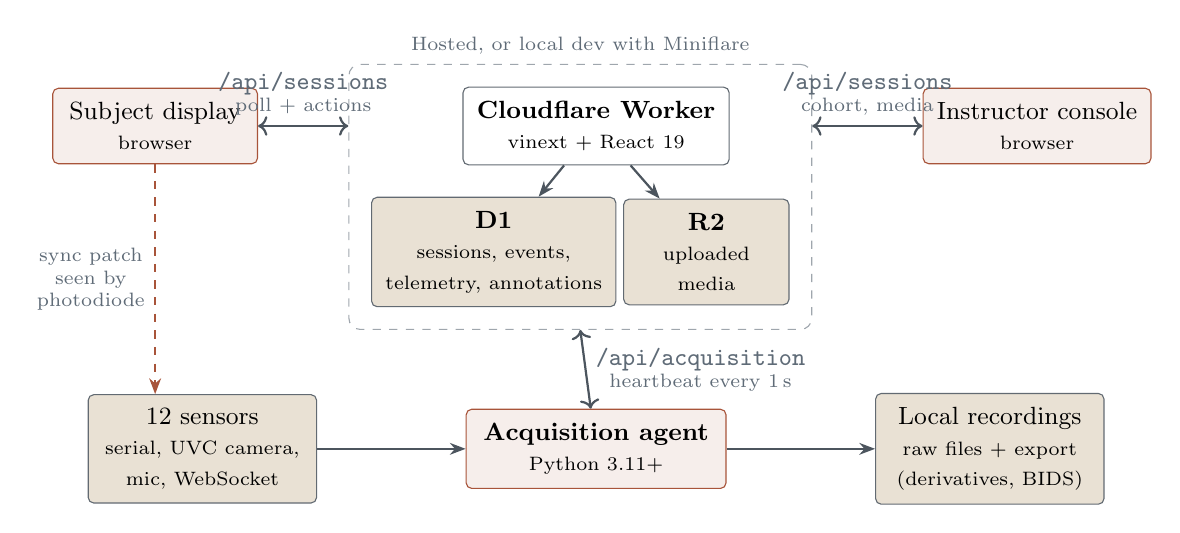
\begin{tikzpicture}[font=\small]
    \node[box,minimum width=3.3cm] (api) at (0,0) {\textbf{Cloudflare Worker}\\\scriptsize vinext + React 19};
    \node[soft,minimum width=2.1cm] (d1) at (-1.3,-1.6) {\textbf{D1}\\\scriptsize sessions, events,\\\scriptsize telemetry, annotations};
    \node[soft,minimum width=2.1cm] (r2) at (1.4,-1.6) {\textbf{R2}\\\scriptsize uploaded\\\scriptsize media};
    \draw[arr] (api) -- (d1);
    \draw[arr] (api) -- (r2);
    \begin{scope}[on background layer]
      \node[group,fit=(api)(d1)(r2),label={[lbl]above:Hosted, or local dev with Miniflare}] (cloud) {};
    \end{scope}
    \node[accent,minimum width=2.6cm] (sub) at (-5.6,0) {Subject display\\\scriptsize browser};
    \node[accent,minimum width=2.6cm] (ins) at (5.6,0) {Instructor console\\\scriptsize browser};
    \node[accent,minimum width=3.3cm] (agent) at (0,-4.1) {\textbf{Acquisition agent}\\\scriptsize Python 3.11+};
    \node[soft,minimum width=2.9cm] (sens) at (-5.0,-4.1) {12 sensors\\\scriptsize serial, UVC camera,\\\scriptsize mic, WebSocket};
    \node[soft,minimum width=2.9cm] (disk) at (5.0,-4.1) {Local recordings\\\scriptsize raw files + export\\\scriptsize (derivatives, BIDS)};
    \draw[arr,<->] (sub) -- node[lbl,above]{\code{/api/sessions}\\poll + actions} (cloud.west |- sub);
    \draw[arr,<->] (ins) -- node[lbl,above]{\code{/api/sessions}\\cohort, media} (cloud.east |- ins);
    \draw[arr,<->] (agent) -- node[lbl,right]{\code{/api/acquisition}\\heartbeat every 1\,s} (cloud.south);
    \draw[arr] (sens) -- (agent);
    \draw[arr] (agent) -- (disk);
    \draw[arr,dashed,clay] (sub.south) -- node[lbl,left]{sync patch\\seen by\\photodiode} (sens.north -| sub.south);
  \end{tikzpicture}
\end{frame}

\begin{frame}{How one sample travels}
  \centering
  \resizebox{\textwidth}{!}{%
  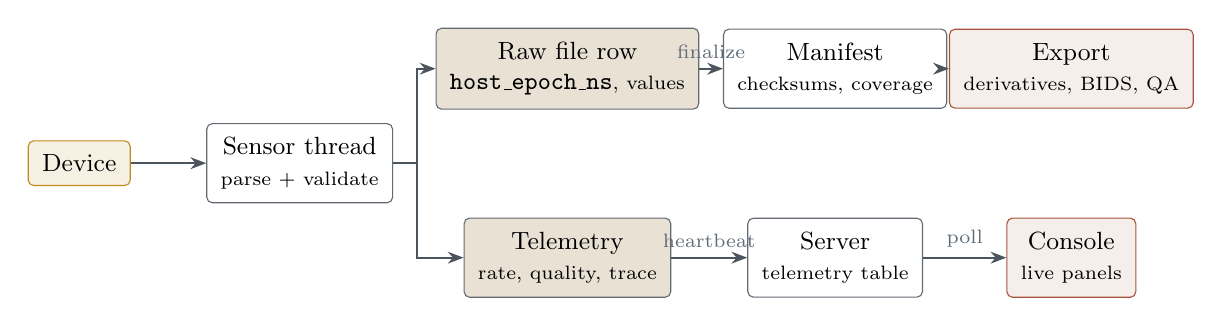
\begin{tikzpicture}[font=\small]
    \node[context] (dev) at (0,0) {Device};
    \node[box] (thread) at (2.8,0) {Sensor thread\\\scriptsize parse + validate};
    \node[soft] (raw) at (6.2,1.2) {Raw file row\\\scriptsize \code{host\_epoch\_ns}, values};
    \node[soft] (tele) at (6.2,-1.2) {Telemetry\\\scriptsize rate, quality, trace};
    \node[box] (manifest) at (9.6,1.2) {Manifest\\\scriptsize checksums, coverage};
    \node[accent] (export) at (12.6,1.2) {Export\\\scriptsize derivatives, BIDS, QA};
    \node[box] (server) at (9.6,-1.2) {Server\\\scriptsize telemetry table};
    \node[accent] (console) at (12.6,-1.2) {Console\\\scriptsize live panels};
    \draw[arr] (dev) -- (thread);
    \draw[arr] (thread.east) -- ++(0.3,0) |- (raw.west);
    \draw[arr] (thread.east) -- ++(0.3,0) |- (tele.west);
    \draw[arr] (raw) -- node[lbl,above]{finalize} (manifest);
    \draw[arr] (manifest) -- (export);
    \draw[arr] (tele) -- node[lbl,above]{heartbeat} (server);
    \draw[arr] (server) -- node[lbl,above]{poll} (console);
  \end{tikzpicture}%
  }
  \vspace{1em}

  \small Raw samples never pass through the browser or the server. The server only sees low-rate telemetry and the protocol events needed to align the raw files.
\end{frame}

\begin{frame}{Technology stack}
  \small
  \begin{tabularx}{\textwidth}{@{}l X@{}}
    \toprule
    \textbf{Layer} & \textbf{Technology} \\
    \midrule
    Web framework & vinext (Next.js App Router API on Vite 8), React 19, TypeScript \\
    Runtime & Cloudflare Workers (Wrangler / Miniflare locally) \\
    Storage & D1 (SQLite): snapshots, event ledger, telemetry, annotations; R2 for media \\
    UI & Tailwind CSS 4, custom editorial styles, Web Worker timers \\
    Agent & Python 3.11+: pyserial, OpenCV (lossless FFV1), sounddevice, websocket-client, NumPy \\
    Optional & pylsl (Lab Streaming Layer output) \\
    Tests & \code{node --test} (esbuild-bundled TypeScript), pytest, hardware emulators \\
    Tooling & ESLint, \code{tsc}, ffmpeg stimulus normalization, Drizzle migrations \\
    \bottomrule
  \end{tabularx}
\end{frame}

\begin{frame}{Repository map: web application}
  \footnotesize
  \begin{tabularx}{\textwidth}{@{}l X@{}}
    \toprule
    \textbf{Path} & \textbf{Responsibility} \\
    \midrule
    \code{app/subject/subject-portal.tsx} & Subject display: clips, ratings, Stroop, N-back, questionnaires, pacers, replay rating, sync patch \\
    \code{app/instructor/editorial-operator-console.tsx} & Instructor console: overview, protocol, review, cohort, recording setup \\
    \code{app/api/sessions}, \code{acquisition}, \code{media} & Session actions, agent channel, media upload \\
    \code{lib/session-engine.ts} & State machine, storage, auto-pause, telemetry merge, export payload \\
    \code{lib/protocol.ts} & Counterbalancing and the step plan with v9 options \\
    \code{lib/stimuli.ts}, \code{tasks.ts}, \code{questionnaires.ts} & Clip registry; Stroop and N-back generators; PANAS, TIPI, NASA-TLX \\
    \code{lib/safety.ts}, \code{lib/rig.ts} & Screening and baseline gate; participant details, artifacts, CSI setup, consent, HR agreement \\
    \code{lib/cohort.ts}, \code{lib/ticker.ts} & Cohort summaries; Web Worker timers \\
    \code{db/}, \code{drizzle/}, \code{tests/} & Schema and migrations; unit and render tests \\
    \bottomrule
  \end{tabularx}
\end{frame}

\begin{frame}{Repository map: acquisition agent}
  \footnotesize
  \begin{tabularx}{\textwidth}{@{}l X@{}}
    \toprule
    \textbf{Path} & \textbf{Responsibility} \\
    \midrule
    \code{meridian\_agent/agent.py} & Main loop: heartbeat, commands (probe, test, calibrate, record, finalize), clock estimate, event log, export \\
    \code{meridian\_agent/sensors.py} & Device drivers: face and thermal cameras, audio, CMS50E, Frontier X ECG, ESP32 CSI / EMG / GSR, respiration, photodiode, environment \\
    \code{meridian\_agent/rppg.py} & Live face-video heart rate (POS method) \\
    \code{meridian\_agent/export.py} & Events, steps, ratings, tasks, questionnaires, annotations, artifacts, QA report, share manifest \\
    \code{meridian\_agent/derivatives.py} & ECG R-peaks and HRV, skin conductance level and responses, breathing rate, audio envelope, face colour trace \\
    \code{meridian\_agent/bids.py}, \code{lsl.py} & BIDS-style export; Lab Streaming Layer output \\
    \code{tools/emulate\_devices.py} & Hardware emulators for testing without sensors \\
    \code{scripts/normalize-media.sh} & Stimulus re-encoding and loudness normalization \\
    \bottomrule
  \end{tabularx}
\end{frame}

% ================================================================ 3
\section{The Twelve Modalities}

\begin{frame}{Modality summary}
  \scriptsize
  \begin{tabularx}{\textwidth}{@{}l l l r l X@{}}
    \toprule
    \textbf{Stream} & \textbf{ID} & \textbf{Device / interface} & \textbf{Rate} & \textbf{Raw file} & \textbf{Main use} \\
    \midrule
    Face video & \code{face} & USB camera (UVC) & 30\,Hz & \code{face.mkv} + frames & rPPG, expressions \\
    Thermal video & \code{thermal} & Thermal camera (UVC, Y16) & 9\,Hz & \code{thermal.mkv} / Y16 raw & Skin temperature \\
    Room audio & \code{audio} & Microphone & 48\,kHz & \code{audio.wav} & Speech, voice arousal \\
    Pulse oximeter & \code{oximeter} & CMS50E, serial & 60\,Hz & \code{oximeter.csv} & HR and SpO$_2$ reference \\
    ECG & \code{ecg} & Frontier X, WebSocket & 125\,Hz & \code{ecg.csv} + packets & Reference HR, HRV \\
    EMG & \code{emg} & ESP32, serial & 1\,kHz & \code{emg.csv} & Muscle activity, motion \\
    EDA / GSR & \code{gsr} & ESP32, JSON lines & 20\,Hz & \code{gsr.csv} & Sympathetic arousal \\
    Respiration & \code{resp} & ESP32 ADC belt & 50\,Hz & \code{resp.csv} & Breathing reference \\
    WiFi CSI (x2) & \code{csi}, \code{csi2} & ESP32 receivers & 100\,Hz & \code{csi.csv} & Contactless vitals \\
    Photodiode & \code{photodiode} & ESP32 ADC & 1\,kHz & \code{photodiode.csv} & Display latency \\
    Environment & \code{environment} & BME280 + light sensor & 1\,Hz & \code{environment.csv} & Room conditions \\
    \bottomrule
  \end{tabularx}
  \vspace{0.4em}

  \footnotesize Every CSV row carries \code{host\_epoch\_ns} and \code{monotonic\_s}; video frames have a per-frame timestamp file.
\end{frame}

\modalityslide{Face video}
{Remote photoplethysmography (tiny skin colour changes with each heartbeat), facial expressions, and head motion. The main contactless target of the dataset.}
{USB camera through OpenCV (V4L2 on Linux, DirectShow on Windows). Resolution and frame rate can be requested; a video file can stand in for testing.}
{\code{face/face.mkv} in lossless FFV1 (decoded frames are bit-identical), \code{face\_frames.csv} with a timestamp and \code{repeated} flag per frame, \code{camera\_settings.json}.}
{Preview, frame rate, dropped frames, whether exposure and white balance were locked, live rPPG heart rate beside ECG and oximeter.}
{Face colour trace and per-step rPPG heart rate (\code{--derive-video}); the trace can be shared when the video is withheld.}
{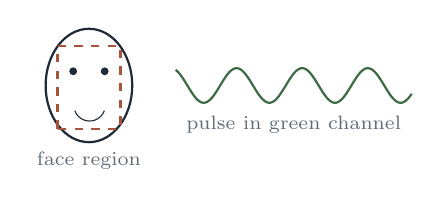
\begin{tikzpicture}
  \draw[ink,thick] (0,0) ellipse (0.55 and 0.72);
  \fill[ink] (-0.2,0.18) circle (0.05) (0.2,0.18) circle (0.05);
  \draw[ink] (-0.18,-0.32) arc (200:340:0.2);
  \draw[clay,dashed,thick] (-0.4,-0.55) rectangle (0.4,0.5);
  \node[lbl] at (0,-0.95) {face region};
  \draw[thick,moss,domain=1.1:4.1,samples=120] plot (\x,{0.22*sin(deg(2*pi*1.2*\x))});
  \node[lbl] at (2.6,-0.5) {pulse in green channel};
\end{tikzpicture}}

\modalityslide{Thermal video}
{Facial skin temperature: nose-tip cooling under stress, warming around the eyes, and nostril temperature changes with breathing.}
{Thermal camera over UVC. With \code{--thermal-format y16} (for example a FLIR Lepton on a PureThermal board) true 16-bit radiometric frames are captured.}
{\code{thermal/thermal.mkv} (lossless), or \code{thermal\_y16.raw} (uint16, centikelvin) with a JSON description; timestamps show flat-field-correction freezes.}
{Colour-mapped preview, frame rate, dropped frames, minimum and maximum temperature.}
{Listed in the BIDS scans file; shared only when thermal sharing is consented.}
{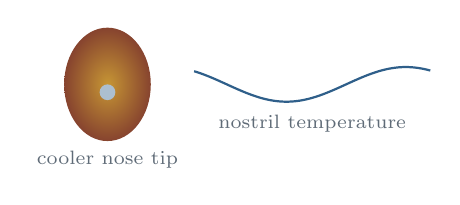
\begin{tikzpicture}
  \shade[inner color=amber!90,outer color=clay!80!black] (0,0) ellipse (0.55 and 0.72);
  \fill[sky!40] (0,-0.1) circle (0.1);
  \node[lbl] at (0,-0.95) {cooler nose tip};
  \draw[thick,sky,domain=1.1:4.1,samples=120] plot (\x,{0.22*sin(deg(2*pi*0.33*\x))});
  \node[lbl] at (2.6,-0.5) {nostril temperature};
\end{tikzpicture}}

\modalityslide{Room audio}
{Speech during the conversation task and the head-movement-and-speaking step; voice features for arousal; a record of what happened in the room.}
{System microphone through sounddevice, mono 16-bit at 48\,kHz.}
{\code{audio/audio.wav}. If the writer falls behind, dropped chunks are filled with silence and counted, so the timeline stays aligned.}
{Audio level meter, sample rate, dropped-audio warnings.}
{A 100\,ms loudness envelope, shareable when the voice recording itself is withheld.}
{\sketch{0.4*sin(3000*\x)*exp(-1*((\x-2.2)^2)/0.8)}{plum}{speech envelope}}

\modalityslide{Pulse oximeter}
{Heart rate, blood oxygen saturation (SpO$_2$), and the fingertip pulse waveform: the contact reference for camera-based heart rate.}
{CMS50E over a USB serial bridge at 115200 baud: 9-byte packets after a start command, with a keep-alive every 5\,s. Detected automatically from its packets.}
{\code{oximeter/oximeter.csv}: SpO$_2$, heart rate, signal strength, and pulse waveform value per packet.}
{Heart rate and SpO$_2$, finger detection, signal strength, rolling waveform; part of the heart-rate agreement panel.}
{Per-step heart rate and SpO$_2$ in \code{physio\_summary.tsv}; BIDS physio file at 60\,Hz.}
{\sketch{0.8*exp(-min(20,((\x-0.83*floor(\x/0.83)-0.18)^2)/0.006))+0.3*exp(-min(20,((\x-0.83*floor(\x/0.83)-0.45)^2)/0.01))}{moss}{fingertip pulse wave}}

\modalityslide{ECG}
{Electrical heart activity: the reference heart rate and beat-to-beat intervals (HRV), used to judge every other heart-rate source.}
{Frontier X chest strap through its live-share WebSocket: packets of 125 samples per second. Duplicate packets and gaps are detected, and device sample times are rebuilt.}
{\code{ecg/ecg.csv} (host time, device sample time, raw count, millivolts, device heart rate) and \code{ecg\_packets.jsonl} (deduplicated source packets).}
{Device heart rate, packet loss, connection health, rolling waveform; part of the heart-rate agreement panel.}
{R-peaks (\code{ecg\_rpeaks.tsv.gz}), per-step heart rate and RMSSD; BIDS physio at 125\,Hz.}
{\sketch{0.9*exp(-min(20,((\x-0.83*floor(\x/0.83)-0.12)^2)/0.0004))-0.2*exp(-min(20,((\x-0.83*floor(\x/0.83)-0.16)^2)/0.001))+0.22*exp(-min(20,((\x-0.83*floor(\x/0.83)-0.42)^2)/0.006))}{clay}{QRS complexes and T waves}}

\modalityslide{EMG}
{Muscle activity (for example the trapezius or facial muscles): exertion, posture changes, speaking, and the motion that contaminates other signals.}
{ESP32 ADC sending \code{t\_us,seq,raw} lines at 1\,kHz over 921600 baud. It answers a \code{?} handshake; gaps in the sequence count as dropped samples.}
{\code{emg/emg.csv}: host time, device microseconds, sequence number, raw ADC value.}
{Raw level, RMS, clipping percentage, sample rate, rolling trace.}
{BIDS physio at 1\,kHz. In the all-modality test RMS rose from 25 at rest to 380 during exertion.}
{\sketch{0.06*sin(2500*\x)+ifthenelse(and(\x>2,\x<3.3),0.6*sin(3100*\x)*abs(sin(700*\x)),0)}{sky}{burst during exertion}}

\modalityslide{EDA / GSR}
{Skin conductance: a slow tonic level plus fast responses driven by sympathetic arousal, for example shortly after an emotional clip starts.}
{ESP32 GSR module sending JSON lines (\code{uS}, \code{raw}, \code{stress}, \code{zScore}) at about 20\,Hz. Detected automatically from the JSON fields.}
{\code{gsr/gsr.csv}: conductance in microsiemens, raw ADC value, stress index, z-score.}
{Conductance, running baseline, z-score, rolling trace; feeds the return-to-baseline gate.}
{Skin conductance level and response count per step; BIDS physio at 20\,Hz.}
{\sketch{0.2+0.04*\x+0.55*(1-exp(-max(0,\x-1.4)/0.3))*exp(-max(0,\x-1.4)/1.3)}{amber}{response after clip onset}}

\modalityslide{Respiration belt}
{Chest or abdominal expansion: the breathing-rate reference for estimates from face video, thermal video, and WiFi CSI.}
{Strain-gauge or conductive-rubber belt on an ESP32 ADC sending \code{t\_us,raw} lines at 50\,Hz; the port is assigned in Recording setup.}
{\code{resp/resp.csv}: host time, device microseconds, raw level.}
{Raw level, live breathing rate in breaths per minute, rolling trace.}
{Per-step breathing rate; BIDS physio at 50\,Hz. Test: 6.1 and 19.9 per minute during the 6 and 20 per minute pacers.}
{\sketch{0.45*sin(deg(2*pi*\x/1.5))}{moss}{breathing cycles}}

\modalityslide{WiFi CSI (two receivers)}
{Channel state information: how the body disturbs the WiFi signal between a transmitter and an ESP32 receiver. Breathing and heartbeat appear as small periodic changes.}
{ESP32 receivers printing \code{CSI\_DATA} lines (timestamp, packet, RSSI, rate, noise, channel, subcarrier amplitudes). Setup records channel, bandwidth, packet rate, and geometry, plus a 60\,s empty-room baseline.}
{\code{csi/csi.csv} and \code{csi2/csi2.csv} (complete raw line), \code{empty\_room} baseline files.}
{RSSI, subcarrier count, amplitude plot, baseline status with packet counts per receiver.}
{BIDS physio with RSSI and all 52 subcarrier amplitudes. Test: breathing found at 5.9 and 20.0 per minute; empty-room variation 10 times lower.}
{
\begin{tikzpicture}[x=1cm,y=0.9cm]
  \draw[sky!50,domain=0:4.5,samples=100] plot (\x,{0.00+0.08*sin(deg(2*pi*\x/1.5))});
  \draw[sky!70,domain=0:4.5,samples=100] plot (\x,{0.28+0.08*sin(deg(2*pi*\x/1.5+40))});
  \draw[sky!85!ink,domain=0:4.5,samples=100] plot (\x,{0.56+0.08*sin(deg(2*pi*\x/1.5+80))});
  \draw[sky!60!ink,domain=0:4.5,samples=100] plot (\x,{0.84+0.08*sin(deg(2*pi*\x/1.5+120))});
  \node[lbl] at (2.3,-0.4) {subcarrier amplitudes};
\end{tikzpicture}}

\modalityslide{Photodiode}
{Light from a small screen-corner patch that flashes when a clip starts or ends and when each step appears: the measured delay between a logged event and what was really on screen.}
{Photodiode on an ESP32 ADC sending \code{t\_us,raw} lines at 1\,kHz. Assigning it turns the patch on in the subject display.}
{\code{photodiode/photodiode.csv}: host time, device microseconds, light level.}
{Light level, minimum and maximum, sample rate.}
{Flash edges matched to display events in \code{sync\_check.tsv}; median, p95, and maximum latency in the QA report.}
{\sketch{ifthenelse(or(and(\x>0.7,\x<0.95),and(\x>2.6,\x<2.85)),0.8,0.05)}{ink}{flashes at display events}}

\modalityslide{Room environment}
{Temperature, humidity, light at the face, and air pressure. Thermal readings and skin conductance depend on the room; lighting changes affect rPPG.}
{BME280 and a light sensor on an ESP32, sending \code{t\_ms,temp\_c,humidity\_pct,lux[,pressure\_hpa]} or JSON at 1\,Hz.}
{\code{environment/environment.csv}.}
{Current temperature, humidity, light, and pressure.}
{Session ranges in the QA report, flagged when lighting changes by more than 30\%; BIDS physio at 1\,Hz.}
{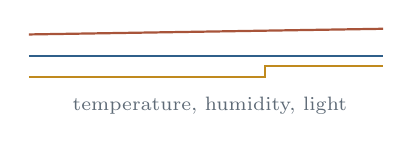
\begin{tikzpicture}[x=1cm,y=0.9cm]
  \draw[clay,thick] (0,0.7) -- (4.5,0.78);
  \draw[sky,thick] (0,0.4) -- (4.5,0.4);
  \draw[amber,thick] (0,0.1) -- (3,0.1) -- (3,0.25) -- (4.5,0.25);
  \node[lbl] at (2.3,-0.3) {temperature, humidity, light};
\end{tikzpicture}}

% ================================================================ 4
\section{The Study Protocol}

\begin{frame}{Session lifecycle}
  \centering
  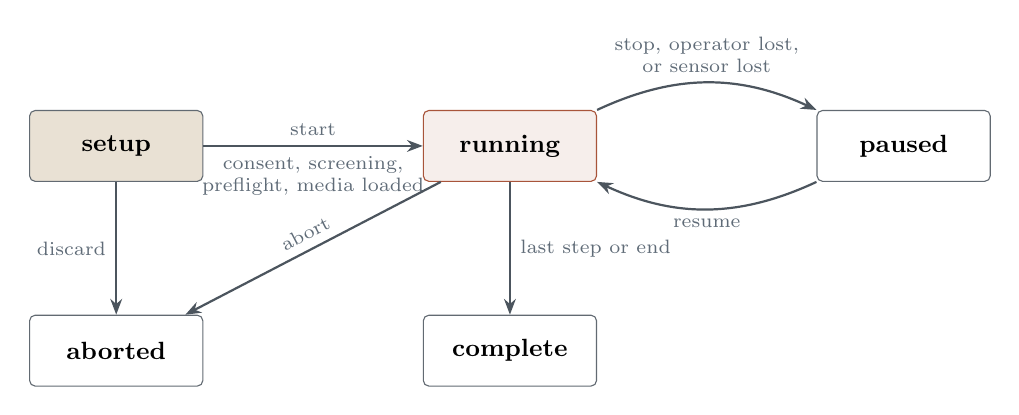
\begin{tikzpicture}[state/.style={box,minimum width=2.2cm,minimum height=9mm}]
    \node[state,fill=sand] (setup) at (0,0) {\textbf{setup}};
    \node[state,accent] (run) at (5,0) {\textbf{running}};
    \node[state] (pause) at (10,0) {\textbf{paused}};
    \node[state] (done) at (5,-2.6) {\textbf{complete}};
    \node[state] (abort) at (0,-2.6) {\textbf{aborted}};
    \draw[arr] (setup) -- node[lbl,above]{start} node[lbl,below]{consent, screening,\\preflight, media loaded} (run);
    \draw[arr] (run.north east) to[bend left=25] node[lbl,above]{stop, operator lost,\\or sensor lost} (pause.north west);
    \draw[arr] (pause.south west) to[bend left=25] node[lbl,below]{resume} (run.south east);
    \draw[arr] (run) -- node[lbl,right]{last step or end} (done);
    \draw[arr] (setup) -- node[lbl,left]{discard} (abort);
    \draw[arr] (run) -- node[lbl,above,sloped]{abort} (abort);
  \end{tikzpicture}
  \vspace{0.6em}

  \small Every transition appends an event to the ledger. Pause time is excluded from step timers.
\end{frame}

\begin{frame}{Protocol v9: 43 steps, about 50 minutes}
  \centering
  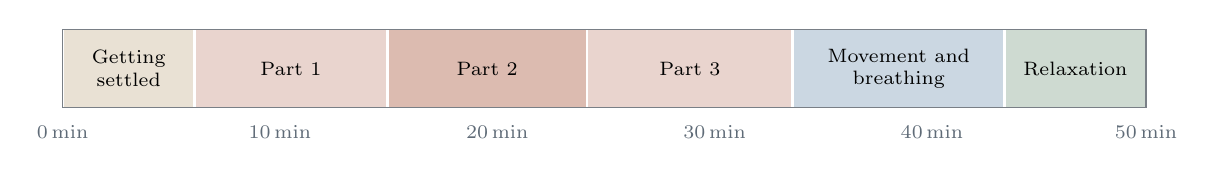
\begin{tikzpicture}[x=0.046mm,y=1mm,font=\scriptsize]
    \foreach \start/\len/\name/\col in {0/365/Getting settled/sand, 365/531/Part 1/clay!25, 896/552/Part 2/clay!40, 1448/568/Part 3/clay!25, 2016/585/Movement and breathing/sky!25, 2601/390/Relaxation/moss!25}{
      \pgfmathsetmacro{\boxwidth}{\len*0.042}
      \pgfmathsetmacro{\boxmid}{\start+\len/2}
      \fill[\col] (\start,0) rectangle ++(\len,10);
      \draw[white,line width=1pt] (\start,0) -- ++(0,10);
      \node[align=center,text width=\boxwidth mm,inner sep=1pt] at (\boxmid,5) {\name};
    }
    \draw[ink!60] (0,0) rectangle (2991,10);
    \foreach \tick/\minutes in {0/0,600/10,1200/20,1800/30,2400/40,2991/50} \node[below,color=slate] at (\tick,-1) {\minutes\,min};
  \end{tikzpicture}
  \vspace{0.6em}

  \footnotesize
  \begin{columns}[T]
    \column{0.5\textwidth}
    \begin{itemize}
      \item Sensor check, PANAS and TIPI questionnaires, eyes-open and eyes-closed baselines
      \item Optional neutral control clip
      \item Three emotion parts: clip, rating, washout, clip, rating, then a task (Stroop or N-back with NASA-TLX, or conversation) and a return-to-baseline gate
    \end{itemize}
    \column{0.5\textwidth}
    \begin{itemize}
      \item Movement and breathing: rest, box breathing, paced breathing at 6, 10, 15, and 20 per minute, breath hold, head movement and speaking, standing, 60\,s exertion, recovery
      \item Body scan, return to normal, PANAS again
      \item Optional replay rating of all clips (about 65 minutes in total)
    \end{itemize}
  \end{columns}
\end{frame}

\begin{frame}{Counterbalancing and stimuli}
  \begin{columns}[T]
    \column{0.5\textwidth}
    \textbf{Emotion order}: six-row Williams square, row $=(\mathit{pid}-1)\bmod 6$
    \vspace{0.2em}

    \scriptsize
    \begin{tabular}{@{}c l@{}}
      \toprule
      Row & Order \\
      \midrule
      1 & happy, sad, disgust, anger, surprise, fear \\
      2 & sad, anger, happy, fear, disgust, surprise \\
      3 & anger, fear, sad, surprise, happy, disgust \\
      4 & fear, surprise, anger, disgust, sad, happy \\
      5 & surprise, disgust, fear, happy, anger, sad \\
      6 & disgust, happy, surprise, sad, fear, anger \\
      \bottomrule
    \end{tabular}
    \vspace{0.3em}

    \small\textbf{Task order}: six permutations, row $=\lfloor(\mathit{pid}-1)/6\rfloor \bmod 6$, so all 36 pairings are covered by 36 participants.
    \column{0.47\textwidth}
    \begin{block}{Stimuli (\code{lib/stimuli.ts})}
      \footnotesize
      \begin{itemize}
        \item Clips: happy 93\,s, fear 95\,s, sad 148\,s, anger 151\,s, disgust 151\,s, surprise 183\,s
        \item All normalized to 1280$\times$720, 30\,fps, $-23$\,LUFS
        \item The registry supports several clips per emotion and a neutral control; each session stores its assigned clips
        \item Downloaded before the start and played from memory
      \end{itemize}
    \end{block}
  \end{columns}
\end{frame}

% ================================================================ 5
\section{Subject Display}

\begin{frame}{Subject display}
  \begin{columns}[T]
    \column{0.5\textwidth}
    \textbf{Screens}
    \begin{itemize}\small
      \item Clips (onset logged when playback actually starts)
      \item Six-part rating: 9-point valence, arousal, dominance; felt emotion and intensity; seen before
      \item Stroop and N-back; questionnaires one item at a time
      \item Fixation, washout, gates, box and paced breathing guides, breath hold (60\,s limit), body scan
      \item Continuous valence-arousal replay rating
    \end{itemize}
    \column{0.5\textwidth}
    \textbf{Behaviour}
    \begin{itemize}\small
      \item Timers follow the server clock (NTP-style offset)
      \item Polling and timers run on a Web Worker, so a hidden display does not stall
      \item Pausing keeps the task on screen; video pauses in place
      \item \code{step\_displayed} logged when each step reaches the screen
      \item Sync patch shown when a photodiode is assigned
      \item Requests retry until the server accepts them
    \end{itemize}
  \end{columns}
\end{frame}

\begin{frame}{Tasks and self-report}
  \begin{columns}[T]
    \column{0.32\textwidth}
    \begin{block}{Stroop}
      \footnotesize 30 seeded trials, 15 congruent and 15 incongruent, no run longer than 3, 400\,ms fixation, 2\,s deadline. Per-trial data and interference cost.
    \end{block}
    \column{0.32\textwidth}
    \begin{block}{N-back}
      \footnotesize 8 practice trials with feedback, then 20 scored trials with exactly 30\% targets and no accidental matches. Hits, false alarms, $d'$.
    \end{block}
    \column{0.32\textwidth}
    \begin{block}{Questionnaires}
      \footnotesize PANAS at the start and end, TIPI at the start, NASA-TLX after each cognitive task. Scored on the server.
    \end{block}
  \end{columns}
  \vspace{0.8em}
  \centering
  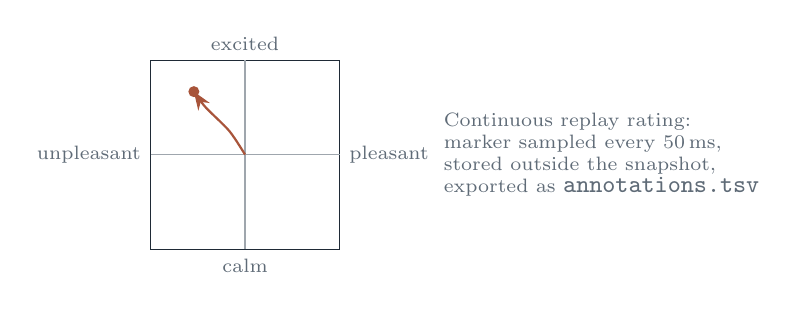
\begin{tikzpicture}[font=\scriptsize]
    \draw[ink] (0,0) rectangle (2.4,2.4);
    \draw[slate!60] (1.2,0) -- (1.2,2.4) (0,1.2) -- (2.4,1.2);
    \node[lbl,above] at (1.2,2.4) {excited};
    \node[lbl,below] at (1.2,0) {calm};
    \node[lbl,left] at (0,1.2) {unpleasant};
    \node[lbl,right] at (2.4,1.2) {pleasant};
    \draw[clay,thick,-{Stealth}] plot[smooth] coordinates {(1.2,1.2) (1.0,1.5) (0.7,1.8) (0.55,2.0)};
    \fill[clay] (0.55,2.0) circle (0.07);
    \node[lbl,align=left,anchor=west] at (3.6,1.2) {Continuous replay rating:\\marker sampled every 50\,ms,\\stored outside the snapshot,\\exported as \code{annotations.tsv}};
  \end{tikzpicture}
\end{frame}

% ================================================================ 6
\section{Instructor Console}

\begin{frame}{Instructor console}
  \begin{columns}[T]
    \column{0.25\textwidth}
    \textbf{Overview}
    \begin{itemize}\scriptsize
      \item Session banner and controls
      \item Recording health
      \item Heart-rate agreement
      \item Live sensor monitor
      \item Messages and artifact buttons
    \end{itemize}
    \column{0.25\textwidth}
    \textbf{Protocol}
    \begin{itemize}\scriptsize
      \item Step list with skipped steps marked
      \item Script and subject cue
      \item Measured gate with override
      \item N-back level, blood pressure
    \end{itemize}
    \column{0.25\textwidth}
    \textbf{Recording setup}
    \begin{itemize}\scriptsize
      \item Devices and required streams
      \item Protocol options
      \item Consent and sharing
      \item Participant details, screening
      \item CSI setup and empty-room baseline
    \end{itemize}
    \column{0.25\textwidth}
    \textbf{Review and cohort}
    \begin{itemize}\scriptsize
      \item Manifest and ledger export
      \item Session status counts
      \item 6$\times$6 order coverage grid
      \item Skin type, sex, age balance
      \item Per-session quality table
    \end{itemize}
  \end{columns}
  \vspace{0.6em}
  \small Operator presence is sent from a Web Worker; if it is lost while running, the session pauses automatically.
\end{frame}

\begin{frame}{Dataset-rig features}
  \footnotesize
  \begin{tabularx}{\textwidth}{@{}l X@{}}
    \toprule
    \textbf{Feature} & \textbf{What it records and why} \\
    \midrule
    Participant details & Fitzpatrick skin type, age band, sex, eyewear, facial hair, makeup, caffeine / nicotine / exercise, heart-rate medication, camera distances. Categories only; written to \code{participants.tsv} \\
    Consent and sharing & Participation (required) and sharing per modality: face, thermal, voice, physiology, CSI, responses, derived features, future research \\
    Safety screening & Six questions; a yes skips breath hold, standing, or exertion and logs why \\
    CSI setup & Channel, bandwidth, packet rate, transmitter and receiver positions; 60\,s empty-room baseline \\
    Artifact labels & Keys T talking, L left seat, O operator in view (on/off); C cough, M movement, D door, P phone (last 3\,s) \\
    Heart-rate agreement & ECG, oximeter, and face-video heart rate side by side; warning above 8\,bpm spread \\
    Return-to-baseline gate & Heart rate and skin conductance within $\max(2\,\mathrm{SD},\text{floor})$ of the resting baseline for 15\,s \\
    \bottomrule
  \end{tabularx}
\end{frame}

% ================================================================ 7
\section{Session Engine and Storage}

\begin{frame}{Session engine and APIs}
  \begin{columns}[T]
    \column{0.5\textwidth}
    \small
    \begin{itemize}
      \item \code{mutateSession(code, action, payload)} for every change, with revision checks and jittered retries
      \item Snapshot and events written in one batch
      \item Heartbeats update only the telemetry row
      \item Server rules: the subject can only finish steps they control, and timers must have elapsed on the server
    \end{itemize}
    \column{0.47\textwidth}
    \scriptsize
    \begin{tabular}{@{}l l@{}}
      \toprule
      D1 table & Contents \\
      \midrule
      \code{sessions} & protocol snapshot \\
      \code{events} & append-only ledger \\
      \code{session\_telemetry} & sensors, agent, presence \\
      \code{annotations} & replay rating samples \\
      \code{media\_assets} & R2 object index \\
      \bottomrule
    \end{tabular}
    \vspace{0.5em}

    \begin{tabular}{@{}l l@{}}
      \toprule
      Endpoint & Caller \\
      \midrule
      \code{/api/sessions} & both portals, cohort \\
      \code{/api/acquisition} & agent: poll, heartbeat, finalize \\
      \code{/api/media} & instructor uploads \\
      \bottomrule
    \end{tabular}
  \end{columns}
\end{frame}

% ================================================================ 8
\section{Acquisition Agent and Synchronization}

\begin{frame}{Agent loop}
  \begin{columns}[c]
    \column{0.46\textwidth}
    \centering
    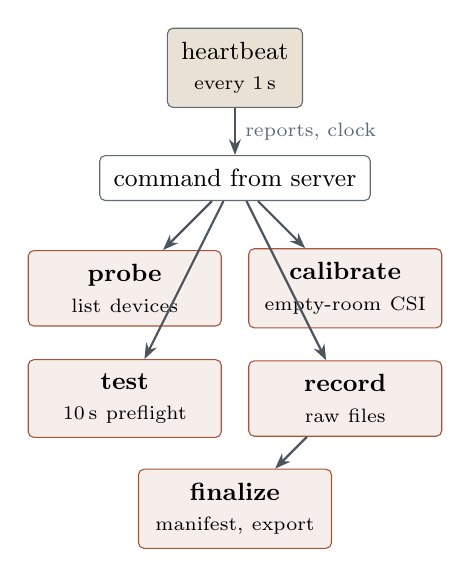
\begin{tikzpicture}[font=\small]
      \node[soft] (hb) at (0,0) {heartbeat\\\scriptsize every 1\,s};
      \node[box] (cmd) at (0,-1.4) {command from server};
      \node[accent,text width=2.1cm] (probe) at (-1.4,-2.8) {\textbf{probe}\\\scriptsize list devices};
      \node[accent,text width=2.1cm] (cal) at (1.4,-2.8) {\textbf{calibrate}\\\scriptsize empty-room CSI};
      \node[accent,text width=2.1cm] (test) at (-1.4,-4.2) {\textbf{test}\\\scriptsize 10\,s preflight};
      \node[accent,text width=2.1cm] (rec) at (1.4,-4.2) {\textbf{record}\\\scriptsize raw files};
      \node[accent,text width=2.1cm] (fin) at (0,-5.6) {\textbf{finalize}\\\scriptsize manifest, export};
      \draw[arr] (hb) -- node[lbl,right]{reports, clock} (cmd);
      \draw[arr] (cmd) -- (probe);
      \draw[arr] (cmd) -- (cal);
      \draw[arr] (cmd) -- (test);
      \draw[arr] (cmd) -- (rec);
      \draw[arr] (rec) -- (fin);
    \end{tikzpicture}
    \column{0.5\textwidth}
    \small
    \begin{itemize}
      \item One thread per sensor; recording continues through network loss
      \item Preflight: required streams good, storage writable, disk space for a full session with margin, clock offset under 100\,ms
      \item Clock offset taken from the fastest of the last 16 exchanges
      \item Video written on its own thread; exposure and white balance locked after warm-up
      \item Stream health judged when recording stops
    \end{itemize}
  \end{columns}
\end{frame}

\begin{frame}{Three clocks, one timeline}
  \centering
  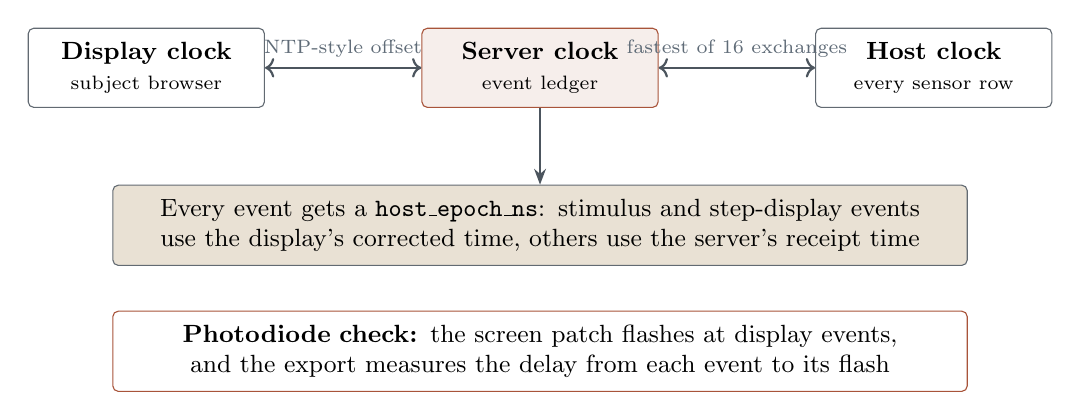
\begin{tikzpicture}[font=\small]
    \node[box,minimum width=3cm] (disp) at (-5,0) {\textbf{Display clock}\\\scriptsize subject browser};
    \node[accent,minimum width=3cm] (srv) at (0,0) {\textbf{Server clock}\\\scriptsize event ledger};
    \node[box,minimum width=3cm] (host) at (5,0) {\textbf{Host clock}\\\scriptsize every sensor row};
    \draw[arr,<->] (disp) -- node[lbl,above]{NTP-style offset} (srv);
    \draw[arr,<->] (srv) -- node[lbl,above]{fastest of 16 exchanges} (host);
    \node[soft,text width=10.5cm] (out) at (0,-2) {Every event gets a \code{host\_epoch\_ns}: stimulus and step-display events use the display's corrected time, others use the server's receipt time};
    \draw[arr] (srv) -- (out);
    \node[box,draw=clay,text width=10.5cm] (pd) at (0,-3.6) {\textbf{Photodiode check:} the screen patch flashes at display events, and the export measures the delay from each event to its flash};
  \end{tikzpicture}
\end{frame}

% ================================================================ 9
\section{Data Output and Quality Control}

\begin{frame}[fragile]{Recording folder and analysis bundle}
  \begin{columns}[T]
    \column{0.47\textwidth}
    \footnotesize
\begin{verbatim}
session_CODE_TIMESTAMP/
  acquisition.json  manifest.json
  session_events.jsonl
  face/  face.mkv  face_frames.csv
  thermal/  audio/  oximeter/
  ecg/  emg/  gsr/  resp/
  csi/  csi2/  (+ empty-room files)
  photodiode/  environment/
  export/
\end{verbatim}
    \column{0.5\textwidth}
    \footnotesize
\begin{verbatim}
export/
  events.tsv  steps.tsv  artifacts.tsv
  ratings.tsv  tasks.tsv
  stroop_trials.tsv  nback_trials.tsv
  questionnaire_items/scores.tsv
  annotations.tsv  sync_check.tsv
  participants.tsv  session.json
  consent.json  share_manifest.json
  qa_report.json  qa_report.md
  derivatives/  bids/
\end{verbatim}
  \end{columns}
\end{frame}

\begin{frame}{Derivatives, BIDS, sharing, and QA}
  \begin{columns}[T]
    \column{0.5\textwidth}
    \begin{block}{\code{derivatives/physio\_summary.tsv} (per step)}
      \footnotesize ECG heart rate and RMSSD, oximeter heart rate and SpO$_2$, skin conductance level and response count, belt breathing rate, face-video heart rate
    \end{block}
    \begin{block}{BIDS-style copy}
      \footnotesize Events with steps and artifacts; physio resampled to nominal rates with JSON sidecars (CSI includes every subcarrier); scans list for video and audio
    \end{block}
    \column{0.47\textwidth}
    \begin{block}{Share manifest}
      \footnotesize Every file marked shareable or withheld according to consent; nothing is shareable without recorded consent
    \end{block}
    \begin{block}{QA report}
      \footnotesize Per step: required-stream coverage, active vs planned time, pauses, restarted clips, artifact seconds. Per session: skipped steps, gates, sync latency, environment, missing details, CSI baseline
    \end{block}
  \end{columns}
\end{frame}

% ================================================================ 10
\section{Testing and Results}

\begin{frame}{Testing approach}
  \begin{columns}[T]
    \column{0.5\textwidth}
    \begin{itemize}\small
      \item \code{npm test}: build plus 27 tests (rendering, counterbalancing, task generators, safety, rig features, stimuli, cohort)
      \item \code{pytest}: 57 agent tests (parsers, auto-detection, lossless video, camera lock, Y16, clock, export, derivatives, BIDS, LSL, photodiode)
      \item ESLint and \code{tsc} clean
    \end{itemize}
    \column{0.47\textwidth}
    \begin{block}{All-modality session}
      \footnotesize
      \begin{itemize}
        \item Real: microphone and one USB serial board (silent, correctly reported)
        \item Emulated over virtual serial ports and a WebSocket: oximeter, ECG, EMG, GSR, respiration, two CSI receivers, photodiode, environment
        \item Cameras: a face video with a known 72\,bpm pulse and a thermal-style video
        \item 11 minutes, all 12 streams, 0\% dropout
      \end{itemize}
    \end{block}
  \end{columns}
\end{frame}

\begin{frame}{All-modality results}
  \centering
  \small
  \begin{tabular}{@{}l l l@{}}
    \toprule
    Check & Generated & Measured in the export \\
    \midrule
    Heart rate at rest, clip, exertion (ECG, oximeter) & 72, 76, 112 & 72, 75, 108 \\
    Breathing during 6 and 20 per minute pacers (belt) & 6, 20 & 6.1, 19.9 \\
    Breathing from WiFi CSI & 6, 20 & 5.9, 20.0 \\
    Face-video heart rate (rPPG) & 72 & 72.1 \\
    EMG RMS, rest vs exertion & low vs bursts & 25 vs 380 \\
    CSI amplitude variation, empty vs occupied & lower when empty & 0.055 vs 0.56 \\
    Photodiode flashes matched & 15 display events & 15 of 15 \\
    Lossless face video & 19,929 frames & 19,929 frames and timestamps \\
    Skin conductance responses & after clip onsets & up to 4 per clip step \\
    \bottomrule
  \end{tabular}
\end{frame}

\begin{frame}{Bugs found by the test, now fixed}
  \small
  \begin{enumerate}
    \item Preflight clock check failed under load because of one delayed heartbeat; it now uses the fastest recent exchange
    \item Complete streams were marked failed because health was judged after hashing a 1.9\,GB video; it is now judged when recording stops
    \item The photodiode check counted 6,272 flashes when flashes were rare; now 15 of 15
    \item The empty-room CSI baseline hid a silent receiver; it now reports packets per receiver
    \item BIDS CSI files held only RSSI; they now include every subcarrier amplitude
    \item A hidden subject display delayed steps by up to 55\,s; polling and timers now run on a Web Worker
  \end{enumerate}
\end{frame}

\begin{frame}{Open items and next steps}
  \begin{columns}[T]
    \column{0.5\textwidth}
    \textbf{Research team}
    \begin{itemize}\small
      \item Review screening questions, gate thresholds, and questionnaire licensing
      \item Register alternative and neutral clips
      \item Pilot with real hardware and a full-length session
    \end{itemize}
    \column{0.5\textwidth}
    \textbf{Engineering}
    \begin{itemize}\small
      \item Firmware for the photodiode, belt, and environment boards
      \item Radiometric thermal and camera lock on the lab devices
      \item Verify the baseline gate with a full 120\,s baseline
      \item Server-sent events instead of polling
    \end{itemize}
  \end{columns}
\end{frame}

\begin{frame}[plain]
  \vfill
  \centering
  {\color{ink}\Huge\bfseries Thank you}\par\vspace{0.5em}
  {\color{clay}\rule{3em}{2pt}}\par\vspace{0.8em}
  {\small\color{slate}Meridian Multimodal Research Platform \quad\textbar\quad Protocol v9}
  \vfill
\end{frame}

\end{document}
